% Prosojnice za predstavitev (približno 10 minut). Prevedba iz te mape (dvakrat, zaradi naslovnice in števila strani):
%   pdflatex prosojnice.tex
\documentclass[aspectratio=169,11pt]{beamer}
\usepackage[T1]{fontenc}
\usepackage[utf8]{inputenc}
\usepackage[scaled=0.92]{helvet}
\usepackage{booktabs}
\usepackage{amsmath}
\usepackage{tikz}
\usetikzlibrary{quantikz2}
\graphicspath{{../img/}}

% ------------------------------------------------------------------ videz
\usetheme{default}
\setbeamersize{text margin left=7mm,text margin right=7mm}
\definecolor{temna}{HTML}{14304F}    % naslovni pas
\definecolor{modra}{HTML}{2A6FBB}    % poudarki
\definecolor{oranzna}{HTML}{D55E00}  % ista barva kot procesor na slikah
\definecolor{siva}{HTML}{5F6B7A}
\definecolor{ozadje}{HTML}{EEF2F7}

\setbeamertemplate{navigation symbols}{}
\setbeamercolor{normal text}{fg=black!88}
\setbeamercolor{frametitle}{fg=white,bg=temna}
\setbeamercolor{crta}{bg=oranzna}
\setbeamerfont{frametitle}{series=\bfseries,size=\large}
\makeatletter
\setbeamertemplate{frametitle}{%
  \nointerlineskip%
  \@tempdima=\textwidth\advance\@tempdima by\beamer@leftmargin\advance\@tempdima by\beamer@rightmargin%
  \begin{beamercolorbox}[wd=\the\@tempdima,ht=3.4ex,dp=1.7ex,leftskip=7mm]{frametitle}%
    \usebeamerfont{frametitle}\insertframetitle%
  \end{beamercolorbox}%
  \nointerlineskip%
  \begin{beamercolorbox}[wd=\the\@tempdima,ht=1.6pt,dp=0pt]{crta}\end{beamercolorbox}%
}
\makeatother
% noga: tanek pas napredka, kratek naslov in številka prosojnice
\setbeamercolor{footline}{fg=siva}
\setbeamerfont{footline}{size=\tiny}
\setbeamertemplate{footline}{%
  {\color{modra}\rule{\dimexpr\paperwidth*\insertframenumber/\inserttotalframenumber\relax}{1.2pt}}%
  \par\nointerlineskip%
  \begin{beamercolorbox}[wd=\paperwidth,ht=2.6ex,dp=1.2ex,leftskip=7mm,rightskip=7mm]{footline}%
    \usebeamerfont{footline}Igra GHZ na procesorju IBM\hfill\insertframenumber\,/\,\inserttotalframenumber%
  \end{beamercolorbox}%
}
\setbeamertemplate{itemize items}[square]
\setbeamertemplate{itemize subitem}{\textbf{--}}
\setbeamertemplate{enumerate items}[circle]
\setbeamercolor{itemize item}{fg=modra}
\setbeamercolor{itemize subitem}{fg=modra}
\setbeamercolor{item projected}{fg=white,bg=modra}
\setbeamertemplate{blocks}[rounded][shadow=false]
\setbeamercolor{block title}{fg=white,bg=modra}
\setbeamercolor{block body}{fg=black!88,bg=ozadje}
\setbeamerfont{block title}{series=\bfseries,size=\normalsize}

\newcommand{\poudari}[1]{\textbf{\textcolor{oranzna}{#1}}}
% ploščica z veliko številko in kratkim opisom: \ploscica[barva]{številka}{opis}
\newcommand{\ploscica}[3][modra]{%
  \begin{tikzpicture}
  \node[fill=ozadje,rounded corners=2.5pt,inner xsep=9pt,inner ysep=5pt,text width=\dimexpr\linewidth-18pt\relax,align=left] (p)
    {\raggedright{\Large\bfseries\color{temna}#2\par}\vspace{1pt}{\footnotesize #3\par}};
  \fill[#1] ([xshift=0pt]p.north west) rectangle ([xshift=3.5pt]p.south west);
  \end{tikzpicture}}

\title{Igra GHZ na procesorju IBM}
\subtitle{Kvantna in klasična strategija ob šumu}
\author{Erik Radovičevič in Dominik Krašovec}
\institute{Skupina 20, NPMP 2026/27}
\date{}

\begin{document}

% ------------------------------------------------------------------ naslovnica
% Okras je del čipa ibm_fez z našim drevesom kubitov za N = 20 (slika v poročilu).
\begin{frame}[plain]
\begin{tikzpicture}[remember picture,overlay]
\fill[temna] (current page.south west) rectangle (current page.north east);
\begin{scope}[shift={([xshift=-78mm,yshift=-7mm]current page.north east)},x=5.1mm,y=5.1mm]
  \foreach \v in {0,...,7} {
    \draw[white,opacity=0.20,line width=0.6pt] (0,-2*\v) -- (15,-2*\v);
    \foreach \s in {0,...,15} \fill[white,opacity=0.30] (\s,-2*\v) circle (1.5pt);
  }
  \foreach \v in {0,2,4,6} \foreach \s in {3,7,11,15} {
    \draw[white,opacity=0.20,line width=0.6pt] (\s,-2*\v) -- (\s,-2*\v-2);
    \fill[white,opacity=0.30] (\s,-2*\v-1) circle (1.5pt);
  }
  \foreach \v in {1,3,5} \foreach \s in {1,5,9,13} {
    \draw[white,opacity=0.20,line width=0.6pt] (\s,-2*\v) -- (\s,-2*\v-2);
    \fill[white,opacity=0.30] (\s,-2*\v-1) circle (1.5pt);
  }
  \draw[oranzna,line width=1.6pt,line cap=round] (5,-8) -- (9,-8) (7,-8) -- (7,-10) (3,-10) -- (11,-10)
      (5,-10) -- (5,-12) -- (4,-12) (9,-10) -- (9,-12);
  \foreach \p in {(5,-8),(6,-8),(7,-8),(8,-8),(9,-8),(7,-9),(3,-10),(4,-10),(5,-10),(6,-10),(8,-10),(9,-10),(10,-10),
                  (11,-10),(5,-11),(9,-11),(4,-12),(5,-12),(9,-12)} \fill[oranzna] \p circle (2.3pt);
  \fill[white] (7,-10) circle (3pt);
  \fill[oranzna] (7,-10) circle (1.7pt);
\end{scope}
\node[anchor=north west,align=left,text=white,font=\bfseries\fontsize{24}{29}\selectfont]
  at ([xshift=11mm,yshift=-20mm]current page.north west) {Igra GHZ\\ na procesorju IBM};
\fill[oranzna] ([xshift=11mm,yshift=-45mm]current page.north west) rectangle ++(22mm,1.1mm);
\node[anchor=north west,align=left,text=white,font=\large]
  at ([xshift=11mm,yshift=-49mm]current page.north west) {Kvantna in klasična strategija ob šumu};
\node[anchor=south west,align=left,text=white!85!temna,font=\small]
  at ([xshift=11mm,yshift=9mm]current page.south west) {Erik Radovičevič in Dominik Krašovec\\ Skupina 20, NPMP 2026/27};
\end{tikzpicture}
\end{frame}

% ------------------------------------------------------------------ 1. igra
\begin{frame}{Igra GHZ}
\begin{columns}[T]
\begin{column}{0.52\textwidth}
\begin{itemize}
\item Igra $N$ igralcev. Sodnik izbere bite $x_1,\dots,x_N$ s \textbf{sodo vsoto}.
\item Igralec $j$ vidi le svoj bit $x_j$ in odgovori z enim bitom $y_j$.
\item Med igro se igralci \poudari{ne smejo pogovarjati}.
\item Zmagajo vsi skupaj, če velja
\[
y_1\oplus\dots\oplus y_N = \frac{x_1+\dots+x_N}{2} \bmod 2 .
\]
\end{itemize}
\end{column}
\begin{column}{0.45\textwidth}
\centering
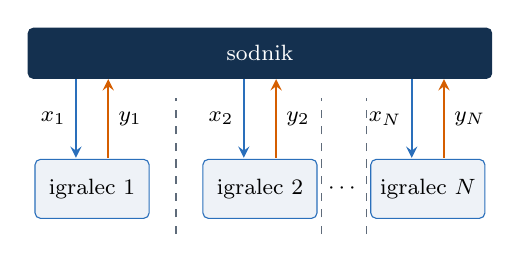
\begin{tikzpicture}[x=0.82cm,y=0.82cm,>=stealth,font=\footnotesize]
\node[rounded corners=2pt,fill=temna,text=white,minimum width=5.9cm,minimum height=0.65cm] at (0,3.4) {sodnik};
\foreach \x/\ime in {-2.6/1,0/2,2.6/N} {
  \node[rounded corners=2pt,fill=ozadje,draw=modra,minimum width=1.45cm,minimum height=0.75cm] at (\x,1.3) {igralec $\ime$};
  \draw[->,thick,modra] (\x-0.25,3.0) -- node[left,text=black] {$x_{\ime}$} (\x-0.25,1.78);
  \draw[->,thick,oranzna] (\x+0.25,1.78) -- node[right,text=black] {$y_{\ime}$} (\x+0.25,3.0);
}
\node at (1.3,1.3) {$\cdots$};
\foreach \x in {-1.3,0.95,1.65} \draw[dashed,siva] (\x,0.6) -- (\x,2.7);
\end{tikzpicture}

\smallskip
{\scriptsize\color{siva} Črtkane črte: igralci med igro ne morejo komunicirati.}
\end{column}
\end{columns}
\medskip
\begin{block}{Primer $N=3$}
Pri vhodu 000 mora biti med odgovori \textbf{sodo} število enic, pri vhodih 110, 101 in 011 pa \textbf{liho}.
\end{block}
\end{frame}

% ------------------------------------------------------------------ 2. vprašanje
\begin{frame}{Raziskovalno vprašanje}
\begin{itemize}
\item Igralci s prepletenimi kubiti lahko zmagajo pogosteje kot z vsako klasično strategijo.
\item Današnji kvantni procesorji pa so \poudari{šumni}: napake nastajajo pri dvokubitnih vratih, med čakanjem kubitov
      in pri branju.
\end{itemize}
\medskip
\begin{block}{Vprašanje}
Do koliko igralcev $N$ kvantna strategija na šumnem procesorju IBM Heron (ibm\_fez, 156 kubitov) v igri GHZ še premaga
najboljšo klasično strategijo in koliko šum pri tem zmanjša delež zmag?
\end{block}
\medskip
\begin{itemize}
\item \textbf{Pričakovanje}: brez šuma je delež zmag 1, šum ga z večanjem $N$ znižuje proti $1/2$. Procesor bi moral
      klasično strategijo premagati tudi pri več deset igralcih.
\end{itemize}
\end{frame}

% ------------------------------------------------------------------ 3. dogovor pred igro
\begin{frame}{Pred igro: dogovor o strategiji}
\centering
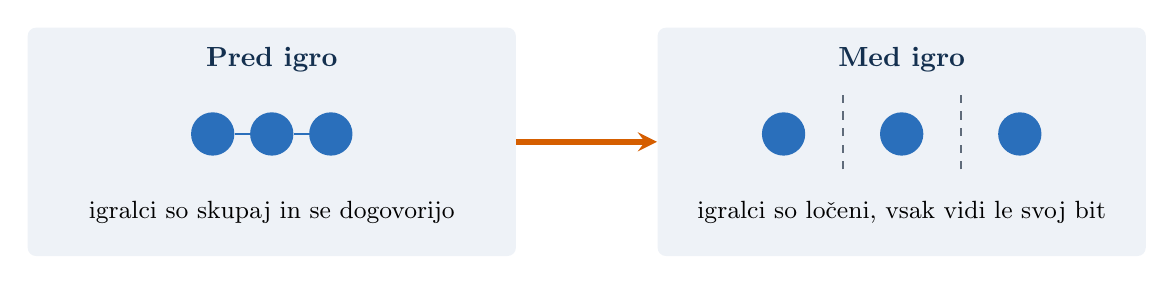
\begin{tikzpicture}[>=stealth,font=\small,igralec/.style={circle,fill=modra,minimum size=5.5mm,inner sep=0pt}]
% pred igro: igralci skupaj
\node[rounded corners=3pt,fill=ozadje,minimum width=6.2cm,minimum height=2.9cm] (pred) at (0,0) {};
\node[font=\bfseries,text=temna] at (0,1.05) {Pred igro};
\node[igralec] (a1) at (-0.75,0.1) {}; \node[igralec] (a2) at (0,0.1) {}; \node[igralec] (a3) at (0.75,0.1) {};
\draw[modra,thick] (a1) -- (a2) -- (a3);
\node at (0,-0.9) {igralci so skupaj in se dogovorijo};
% med igro: igralci ločeni
\node[rounded corners=3pt,fill=ozadje,minimum width=6.2cm,minimum height=2.9cm] (med) at (8.0,0) {};
\node[font=\bfseries,text=temna] at (8.0,1.05) {Med igro};
\foreach \x/\j in {6.5/1,8.0/2,9.5/3} {
  \node[igralec] (b\j) at (\x,0.1) {};
}
\foreach \x in {7.25,8.75} \draw[dashed,siva,thick] (\x,-0.35) -- (\x,0.6);
\node at (8.0,-0.9) {igralci so ločeni, vsak vidi le svoj bit};
\draw[->,line width=2pt,oranzna] (pred) -- (med);
\end{tikzpicture}

\bigskip
\begin{columns}[T]
\begin{column}{0.47\textwidth}
\begin{block}{Klasična strategija}
Vsak igralec vnaprej ve, kako bo odgovoril na bit 0 in kako na bit 1.
\end{block}
\end{column}
\begin{column}{0.47\textwidth}
\begin{block}{Kvantna strategija}
Igralci pred igro prepletejo svoje kubite. Vsak odnese en kubit skupnega stanja GHZ.
\end{block}
\end{column}
\end{columns}
\end{frame}

% ------------------------------------------------------------------ 4. klasična strategija
\begin{frame}{Klasična strategija}
\begin{columns}[T]
\begin{column}{0.49\textwidth}
\begin{itemize}
\item Vsak igralec ima le štiri možnosti: vedno odgovori 0, vedno 1, ponovi svoj bit ali ga obrne.
\item \textbf{Primer $N=3$}: vsi trije vedno odgovorijo 1. Zmagajo pri vhodih 110, 101 in 011, izgubijo pri 000.
      Verjetnost zmage je \poudari{3/4}.
\item Splošna meja (Brassard, Broadbent in Tapp, 2005):
\[
p_\text{klas}(N) = \frac{1}{2} + 2^{-\lceil N/2\rceil}
\]
\item Že pri $N=10$ je le 0,53, pri $N\ge30$ pa manj kot 0,5001.
\end{itemize}
\end{column}
\begin{column}{0.48\textwidth}
\begin{block}{Zakaj pri $N=3$ ne gre bolje od $3/4$}
\small
Igralec $j$ odgovori $a_j$ na bit 0 in $b_j$ na bit 1. Za zmago pri vseh štirih vhodih bi moralo veljati:
\[
\begin{aligned}
\text{vhod 000:}\quad & a_1\oplus a_2\oplus a_3 = 0\\
\text{vhod 110:}\quad & b_1\oplus b_2\oplus a_3 = 1\\
\text{vhod 101:}\quad & b_1\oplus a_2\oplus b_3 = 1\\
\text{vhod 011:}\quad & a_1\oplus b_2\oplus b_3 = 1
\end{aligned}
\]
Seštejemo vse štiri. Na levi se vsak bit pojavi dvakrat, zato je vsota 0. Na desni je $0\oplus1\oplus1\oplus1=1$.
Vsaka strategija torej izgubi pri vsaj enem vhodu.
\end{block}
\end{column}
\end{columns}
\end{frame}

% ------------------------------------------------------------------ 5. kvantna strategija
\begin{frame}{Kvantna strategija}
\begin{columns}[T]
\begin{column}{0.55\textwidth}
\small
\begin{enumerate}
\setlength{\itemsep}{3pt}
\item Pred igro: stanje GHZ
      $\tfrac{1}{\sqrt2}\bigl(\ket{0\dots0}+\ket{1\dots1}\bigr)$.
\item Igralec z $x_j=1$ izvede \textbf{vrata S}. Ta člen $\ket{1\dots1}$ pomnožijo z $i$: stanje se na krogli zasuče
      za \poudari{$90^\circ$}.
\item Naj bo $k$ število igralcev z bitom 1 ($k$ je sodo). Če je $k$ deljiv s 4, stanje ostane GHZ$^{+}$, sicer
      nastane GHZ$^{-}$ (zasuk za $180^\circ$).
\item Vsi izvedejo \textbf{vrata H}. Nastane enakomerna superpozicija nizov z \textbf{isto pariteto}:
      \begin{itemize}
      \item iz GHZ$^{+}$ vsi nizi s sodim številom enic
      \item iz GHZ$^{-}$ vsi nizi z lihim številom enic
      \end{itemize}
\item \textbf{Meritev} izbere enega od teh nizov. Pariteta odgovorov je zato vedno prava: igralci
      \poudari{vedno zmagajo}.
\end{enumerate}
\end{column}
\begin{column}{0.43\textwidth}
\centering
\begin{quantikz}[row sep=0.2cm, column sep=0.28cm,
  execute at end picture={
    % napisa nad vezjem: levo od črtkane črte priprava stanja GHZ, desno poteze igralcev
    \node[above=4pt,font=\scriptsize\bfseries,text=temna] at (\tikzcdmatrixname-1-3.north |- \tikzcdmatrixname-1-6.north) {pred igro};
    \node[above=4pt,font=\scriptsize\bfseries,text=temna] at (\tikzcdmatrixname-1-6.north) {med igro};
  }]
\lstick{$x_1=1$} & \gate{H} & \ctrl{1} & \ctrl{2}\slice[style={siva,dashed,thick}]{} & \gate[style={fill=oranzna!25}]{S} & \gate{H} & \meter{} \\
\lstick{$x_2=1$} & \qw      & \targ{}  & \qw      & \gate[style={fill=oranzna!25}]{S} & \gate{H} & \meter{} \\
\lstick{$x_3=0$} & \qw      & \qw      & \targ{}  & \qw      & \gate{H} & \meter{}
\end{quantikz}

{\scriptsize\color{siva} Vezje za $N=3$ in vhod $(1,1,0)$.}

\vspace{-2pt}
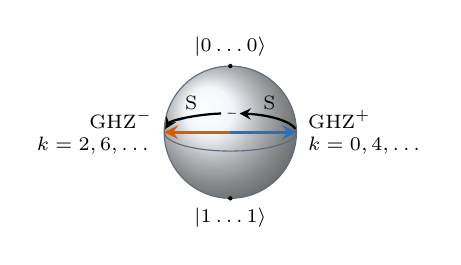
\begin{tikzpicture}[>=stealth,font=\scriptsize,scale=0.8]
\shade[ball color=ozadje,opacity=0.9] (0,0) circle (1.05);
\draw[siva] (0,0) circle (1.05);
\draw[dashed,siva] (1.05,0) arc (0:180:1.05 and 0.3);
\draw[siva] (-1.05,0) arc (180:360:1.05 and 0.3);
\fill (0,1.05) circle (1pt) (0,-1.05) circle (1pt);
\node[above] at (0,1.05) {$\ket{0\dots0}$};
\node[below] at (0,-1.05) {$\ket{1\dots1}$};
\draw[->,very thick,modra] (0,0) -- (1.05,0);
\draw[->,very thick,oranzna] (0,0) -- (-1.05,0);
\node[right,align=left] at (1.08,0) {GHZ$^{+}$\\$k=0,4,\dots$};
\node[left,align=right] at (-1.08,0) {GHZ$^{-}$\\$k=2,6,\dots$};
\draw[->,thick] (1.034,0.052) arc (10:82:1.05 and 0.3);
\draw[->,thick] (-0.146,0.297) arc (98:170:1.05 and 0.3);
\node at (0.62,0.47) {S};
\node at (-0.62,0.47) {S};
\end{tikzpicture}

\vspace{-3pt}
{\scriptsize Po vratih H pri $N=3$:\\[-1pt]
GHZ$^{+}\rightarrow$ 000, 011, 101, 110\\[-2pt]
GHZ$^{-}\rightarrow$ 001, 010, 100, 111}
\end{column}
\end{columns}
\end{frame}

% ------------------------------------------------------------------ 6. poskusi
\begin{frame}{Poskusi s kvantno strategijo}
\begin{columns}[T]
\begin{column}{0.51\textwidth}
\small
\begin{itemize}
\setlength{\itemsep}{2pt}
\item \textbf{Število igralcev}: $N=3$, 5, 10, 20, 30, 40 in 50, na procesorju še 60 in 75.
\item \textbf{Tri izvedbe} z istimi vhodi (8 na vsak $N$):
  \begin{itemize}
  \item idealni simulator: brez napak
  \item šumni simulator: posnetek napak ibm\_fez
  \item procesor ibm\_fez: dve meritvi, 1000 ponovitev vsakega vezja
  \end{itemize}
\item \textbf{Šumni simulator} v vsaki ponovitvi naključno doda tri vrste napak:
\end{itemize}
\centering
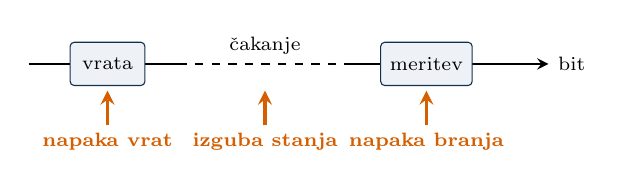
\begin{tikzpicture}[>=stealth,font=\scriptsize,x=1cm,y=1cm]
\draw[thick] (0,0) -- (1.9,0);
\draw[thick,dashed] (1.9,0) -- (4.1,0);
\draw[thick,->] (4.1,0) -- (6.6,0);
\node[rounded corners=1.5pt,draw=temna,fill=ozadje,minimum width=0.95cm,minimum height=0.55cm] at (1.0,0) {vrata};
\node[above] at (3.0,0) {čakanje};
\node[rounded corners=1.5pt,draw=temna,fill=ozadje,minimum width=1.05cm,minimum height=0.55cm] at (5.05,0) {meritev};
\node[right] at (6.6,0) {bit};
\foreach \x/\opis in {1.0/{napaka vrat},3.0/{izguba stanja},5.05/{napaka branja}} {
  \draw[->,oranzna,very thick] (\x,-0.78) -- (\x,-0.34);
  \node[below,text=oranzna,font=\scriptsize\bfseries] at (\x,-0.75) {\opis};
}
\end{tikzpicture}

\end{column}
\begin{column}{0.47\textwidth}
\centering
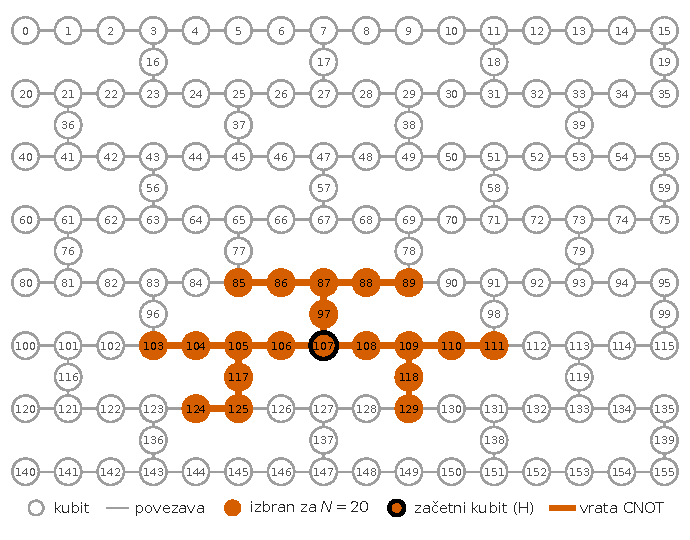
\includegraphics[width=0.94\linewidth]{ibm_fez_cip}

\vspace{-2pt}
{\scriptsize\color{siva} Procesor ibm\_fez, 156 kubitov. Vrata CNOT po povezavah čipa tvorijo drevo.\\[-1pt]
Kubite izberemo po objavljenih napakah (oranžno: $N=20$).}
\end{column}
\end{columns}
\end{frame}

% ------------------------------------------------------------------ 7. rezultat
\begin{frame}{Rezultat: delež zmag v odvisnosti od $N$}
\begin{columns}[c]
\begin{column}{0.57\textwidth}
\centering
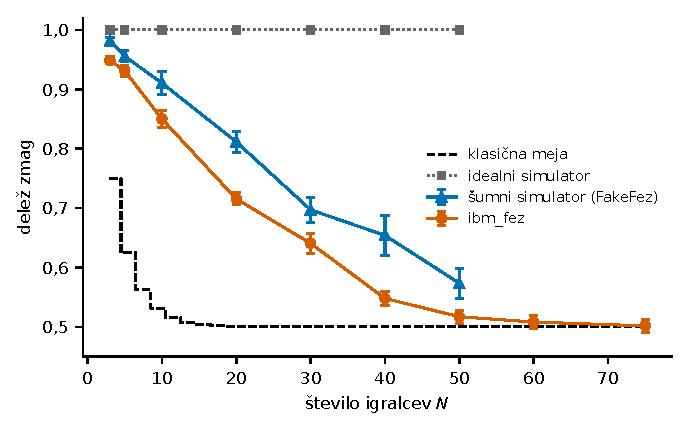
\includegraphics[width=\linewidth]{ghz_igra}

{\footnotesize\color{siva} Kriterij za zmago nad klasično strategijo: $p_\text{ibm}-2\sigma>p_\text{klas}$}
\end{column}
\begin{column}{0.4\textwidth}
\ploscica[modra]{do 40 igralcev}{nad klasično mejo v obeh meritvah}

\vspace{1pt}
\ploscica[oranzna]{50 in 60 igralcev}{nad mejo le v eni od dveh meritev}

\vspace{1pt}
\ploscica[siva]{75 igralcev}{v nobeni meritvi}

\smallskip
\small
\begin{itemize}
\item Idealni simulator vedno zmaga.
\item Na procesorju delež zmag pada z 0,95 pri treh igralcih proti $1/2$.
\item Na procesorju \textbf{nismo uporabili} postopkov za zatiranje napak.
\end{itemize}
\end{column}
\end{columns}
\end{frame}

% ------------------------------------------------------------------ 8. vpliv šuma
\begin{frame}{Vpliv šuma}
\begin{columns}[T]
\begin{column}{0.58\textwidth}
\begin{itemize}
\item Šum zniža delež zmag z 1 na \poudari{0,949} pri treh, \poudari{0,715} pri dvajsetih in \poudari{0,517} pri
      50 igralcih (prva meritev).
\item \textbf{Zakaj}: vsaka napaka, ki obrne izid enega kubita, obrne tudi izid igre. Pri veliko kubitih gre delež
      zmag zato proti $1/2$.
\item \textbf{Viri napak}: napake vrat, izguba stanja med čakanjem in napake branja. Njihovih deležev nismo ločevali.
\item \textbf{Šumni simulator} pokaže padec, a je pri vseh $N$ preveč optimističen.
\end{itemize}
\end{column}
\begin{column}{0.4\textwidth}
\centering
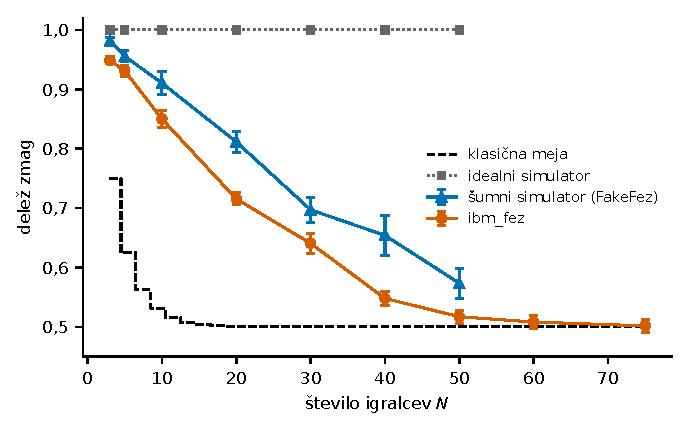
\includegraphics[width=\linewidth]{ghz_igra}

\smallskip
\ploscica[oranzna]{0,02 do 0,14}{za toliko je delež zmag na šumnem simulatorju večji kot na procesorju}
\end{column}
\end{columns}
\end{frame}

% ------------------------------------------------------------------ 9. kaj zmaga pokaže, kaj ni delovalo
\begin{frame}{Kaj rezultat pomeni in kaj ni delovalo}
\begin{columns}[T]
\begin{column}{0.48\textwidth}
\begin{block}{Kaj pomeni zmaga nad klasično mejo}
\begin{itemize}
\item Brez prepletenosti igralci klasične meje ne morejo preseči. Kubiti procesorja so bili torej kljub šumu
      \textbf{prepleteni}.
\item Pravila igre veljajo: po začetku igre med kubiti ni nobenih vrat. Prepletenost ni komunikacija.
\item Ne pokaže pa, da je bilo prepletenih vseh $N$ kubitov hkrati.
\end{itemize}
\end{block}
\end{column}
\begin{column}{0.48\textwidth}
\begin{block}{Kaj ni delovalo: šumna simulacija}
\begin{itemize}
\item S polnim šumnim modelom se simulacija \textbf{ni končala}.
\item Popravek: napake dvokubitnih vrat smo zapisali preprosteje, napake branja pa dodali po simulaciji.
\item Tako je delovala do $N=50$. Pri $N=60$ se v več kot eni uri ni končala.
\end{itemize}
\end{block}
\end{column}
\end{columns}
\medskip
\begin{itemize}
\item \textbf{Omejitve}: le dve meritvi in 8 vhodov na vsak $N$. Izbira kubitov ni izločila slabega kubita 148 (izid 1
      le v \poudari{33~\%} ponovitev), zato smo ga v drugi meritvi izločili.
\end{itemize}
\end{frame}

% ------------------------------------------------------------------ 10. zaključek
\begin{frame}{Zaključek}
\begin{columns}[T]
\begin{column}{0.36\textwidth}
\ploscica[modra]{do 40 igralcev}{kvantna strategija na ibm\_fez premaga najboljšo klasično v obeh meritvah}

\medskip
\ploscica[oranzna]{proti 1/2}{delež zmag pada z naraščajočim $N$}
\end{column}
\begin{column}{0.61\textwidth}
\small
\begin{itemize}
\setlength{\itemsep}{1pt}
\item Pri 50 in 60 igralcih zmaga v eni od dveh meritev, pri 75 v nobeni.
\item Šum zniža delež zmag z 0,95 pri treh na 0,55 pri 40 igralcih.
\item Šumni simulator pokaže potek, a je preveč optimističen.
\end{itemize}
\vspace{-3pt}
\begin{block}{Kako bi delo nadaljevali}
\begin{enumerate}
\setlength{\itemsep}{1pt}
\item Pri izbiri izločiti kubite z veliko objavljeno napako branja.
\item Pri 50 in 60 igralcih uporabiti več vhodov in več ponovitev: tam je delež zmag preblizu $1/2$.
\item Meriti tudi med 40 in 60 igralci in tako natančneje določiti mejo.
\end{enumerate}
\end{block}
\end{column}
\end{columns}
\end{frame}

\end{document}
